
\chapter{LLM with Retrieval-Augmented Generation (RAG)}
Retrieval-Augmented Generation (RAG) is a powerful approach that enhances language models by incorporating external knowledge retrieval. This chapter guides the user through setting up and using RAG, with practical examples.

{\bf Introduction to RAG}
Traditional LLMs rely solely on their pre-trained knowledge. RAG extends this by searching a document database for relevant context before generating a response. This improves accuracy, factuality, and adaptability to domain-specific knowledge.

\begin{figure}[ht]
    \centering
    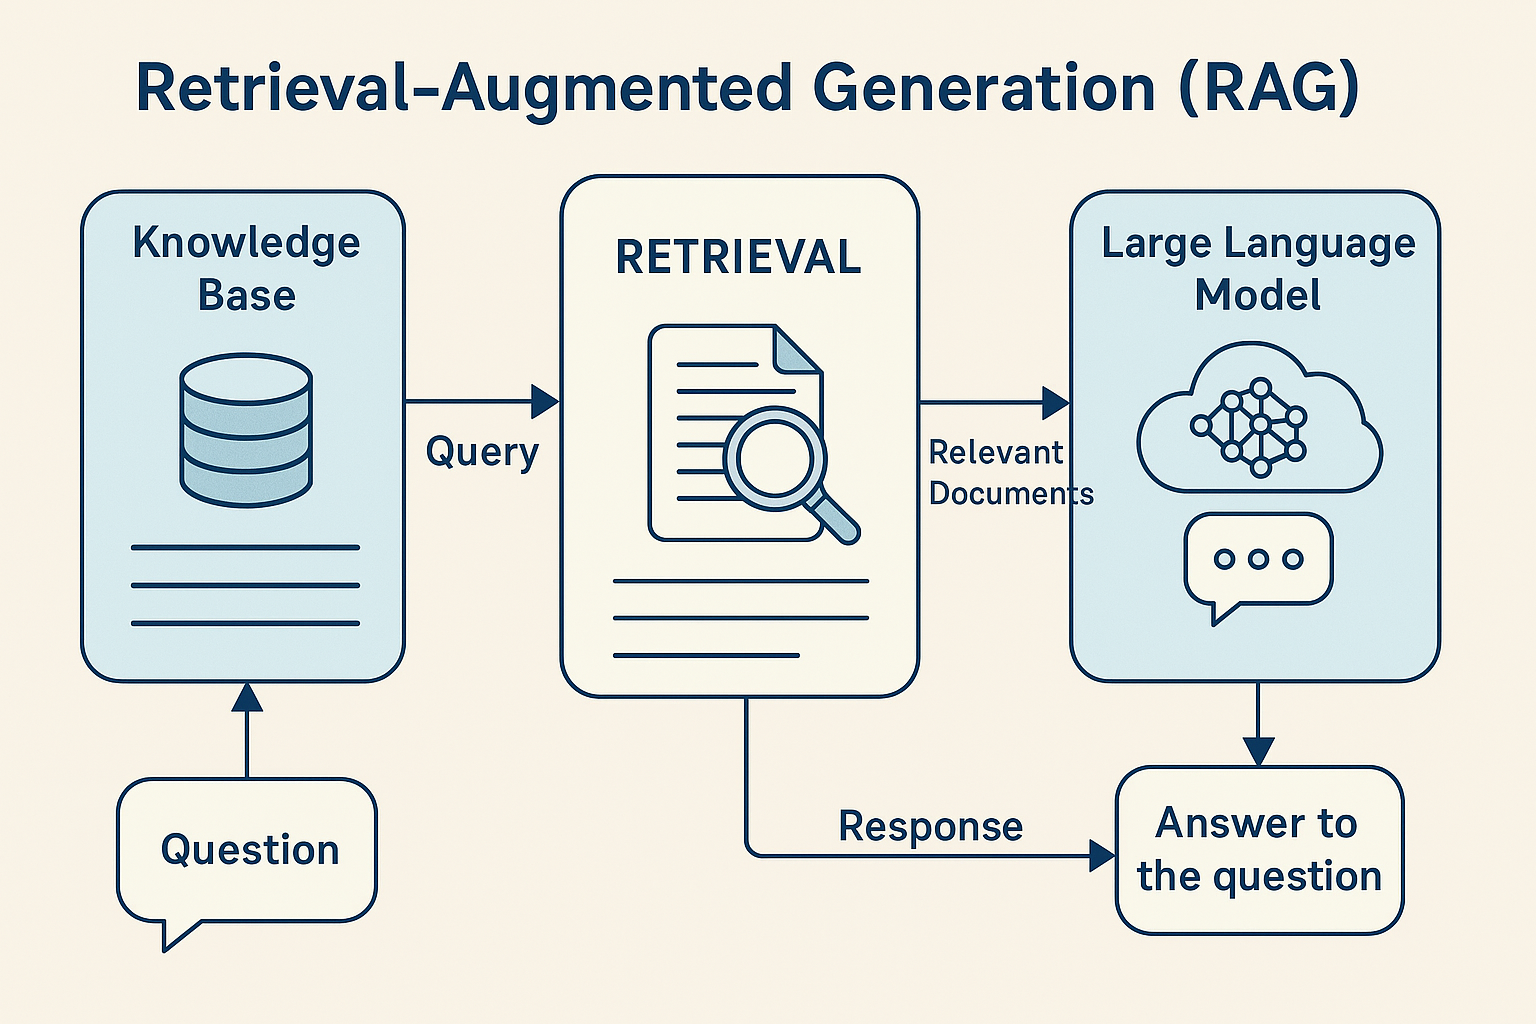
\includegraphics[width=0.7\textwidth]{images/RAG.png}
    \caption{Retrieval-Augmented Generation (RAG) employs the intelligence of Large Language Models (LLM) in combination with local knowledge and databases.}
    \label{fig:vectordb_out}
\end{figure}

%==============================================================================
%
%==============================================================================
\section{Preparing Documents}


{\bf Installing Required Dependencies}
To set up RAG, install the necessary libraries:

\begin{codeonly}{Install Dependencies}
!pip install sentence-transformers==2.2.2 transformers==4.31.0
!pip install faiss-cpu openai numpy pymupdf
\end{codeonly}
To get compatible versions of transformers and sentence-transformers might be a little tricky. I had to go back to python3.11 to get this running in a special virtual environment. 

First, let us work with documents which are in a folder tree starting with its root node \texttt{documents/}. 
We start by recursively loading text and PDF documents from this folder, marching through the tree. For pdf documents, we will use some standard tools to extract the text from the documents - there are more sophisticated packages, but we put simplicity first for the moment.  

\begin{codeonly}{Loading Documents}
import numpy as np
import os
import fitz  # PyMuPDF for PDF text extraction

# Function to extract text from PDF
def extract_text_from_pdf(pdf_path):
    doc = fitz.open(pdf_path)
    text = ""
    for page in doc:
        text += page.get_text()
    return text

# Load documents from a folder recursively
def load_documents_from_folder(folder_path):
    documents = []
    file_info = []
    
    for dirpath, dirnames, filenames in os.walk(folder_path):
        # Exclude .git directories
        dirnames[:] = [d for d in dirnames if not d.startswith('.git')]

        for filename in filenames:
            if filename.startswith('.git'):
                continue  # Skip any .git files

            file_path = os.path.join(dirpath, filename)
            if filename.endswith(('.f90','.txt', '.org', '.sh', '.toml','.pdf')) \
                or '.' not in filename:  # Load .txt, .sh, .pdf, and files without extensions
                try:
                    if filename.endswith('.pdf'):
                        content = extract_text_from_pdf(file_path)
                    else:
                        with open(file_path, 'r', encoding='utf-8') as file:
                            content = file.read()
                    documents.append(content)
                    file_info.append((filename, file_path))
                    print(f"Added to DB: {file_path}")
                except Exception as e:
                    print(f"Failed to process {file_path}: {e}")
    
    return documents, file_info
\end{codeonly}

We call the function to load all available documents by 

\begin{codeonly}{Loading Documents}
folder_path = './documents'  # Replace with your folder path
documents, file_info = load_documents_from_folder(folder_path)
\end{codeonly}

As an example we checkout the publically available ICON model by
\begin{codeonly}{Checkout ICON model}
git clone git@gitlab.dkrz.de:icon/icon-model.git
\end{codeonly}

In this case, the output is
\begin{codeonly}{ICON model from icon-model.org loaded}
Added to DB: ./documents/configure
Added to DB: ./documents/make_runscripts
Added to DB: ./documents/utils/install-sh
Added to DB: ./documents/utils/move_to_prefix.sh
Added to DB: ./documents/utils/patch_namelist
Added to DB: ./documents/utils/timewarp
Added to DB: ./documents/utils/icon_sorted_deps.sh
Added to DB: ./documents/utils/id++
Added to DB: ./documents/utils/filelock
Added to DB: ./documents/utils/mkexp/namelist2config
Added to DB: ./documents/utils/mkexp/mkexp
Added to DB: ./documents/utils/mkexp/upexp
Added to DB: ./documents/utils/mkexp/unmergeconfig
Added to DB: ./documents/utils/mkexp/selconfig
Added to DB: ./documents/utils/mkexp/importexp
Added to DB: ./documents/utils/mkexp/editexp
...
\end{codeonly}




%==============================================================================
%
%==============================================================================
\section{Generating Embeddings for Documents}

To retrieve relevant information, we transform text into \textbf{numerical embeddings} using a \textbf{transformer model}. These embeddings capture the \textit{semantic meaning} of text, allowing for similarity-based retrieval and efficient search operations. A widely used approach for generating such embeddings is \textbf{sentence transformers}, which map textual data into a high-dimensional vector space.

In the following implementation, we utilize the \texttt{all-MiniLM-L6-v2} model from the \texttt{sentence-transformers} library. This model provides a compact yet efficient method for encoding textual information. The embeddings are computed using \textbf{mean pooling} over the token representations, ensuring that the vector captures the full meaning of the sentence. Additionally, we apply \textbf{L2 normalization} to facilitate cosine similarity comparisons.

\begin{codeonly}{Generating Embeddings}
from sentence_transformers import SentenceTransformer

embedder = SentenceTransformer('all-MiniLM-L6-v2')

# Load documents and create embeddings
documents, file_info = load_documents_from_folder("documents/")
embeddings = embedder.encode(documents, convert_to_numpy=True)

# Sanity check
print("Loaded documents:", len(documents))
print("Embedding shape:", embeddings.shape)
print("Example file:", file_info[0])
print("Example snippet:\n", documents[0][:200])
\end{codeonly}

The function \texttt{embedder.encode} tokenizes the input text, processes it through the transformer model, and computes a \textbf{mean-pooled representation} over the token dimension. The final embeddings are \textbf{normalized}, ensuring that similarity computations (e.g., cosine similarity) remain well-scaled.

Such embeddings enable applications in \textbf{semantic search}, \textbf{clustering}, and \textbf{document classification} by mapping textual data into a structured numerical space that can be efficiently queried.

In our case we obtain
\begin{codeonly}{Check embeddings}
Loaded documents: 2391
Embedding shape: (2391, 384)
Example file: ('make_runscripts', 'documents/make_runscripts')
Example snippet:
 #! /bin/bash

# ICON
#
# ------------------------------------------
# Copyright (C) 2004-2024, DWD, MPI-M, DKRZ, KIT, ETH, MeteoSwiss
# Contact information: icon-model.org
# See AUTHORS.TXT for a list
\end{codeonly}

Our embeddings variable has a shape of (2391, 384), which means there are 
2391 rows, i.e.\ 2391 text inputs (documents, sentences, or paragraphs). We have
384 columns, i.e.\ each text input is represented as a 384-dimensional vector.

{\bf How the Embeddings Work.}
The closer two embeddings are (e.g., using cosine similarity), the more semantically similar their corresponding texts are.
The high-dimensional space (384D) allows the model to capture complex semantic relationships between texts.

\bigskip
{\bf Retrieving Relevant Documents}
When a user asks a question, we find the most relevant documents by searching the FAISS index.

\begin{codeonly}{Querying the Vector Database}
def query_vector_db(query, k=2):
    query_embedding = get_embedding(query)
    distances, indices = index.search(query_embedding, k)
    return [documents[idx] for idx in indices[0]]

query = "What is the main functionality of BACY?"
retrieved_docs = query_vector_db(query)
print(retrieved_docs)
\end{codeonly}

{\bf Setting Up a Vector Database with FAISS}
To efficiently search for similar text embeddings, we store them in a {\bf FAISS index}. FAISS (Facebook AI Similarity Search) is an optimized library for fast {\bf nearest neighbor search} in high-dimensional spaces. Instead of performing a brute-force comparison of all pairs of embeddings, FAISS allows us to {\em index and retrieve} the most relevant embeddings efficiently.

FAISS supports different types of indexes, but the most basic and commonly used one is 
\textbf{IndexFlatL2}, which stores vectors and enables fast \textit{k}-nearest neighbor (KNN) search using the {\em L2 (Euclidean) distance}.

\begin{codeonly}{Setting Up FAISS Index}
import faiss

# Create FAISS index
dimension = embeddings.shape[1]
index = faiss.IndexFlatL2(dimension)
index.add(embeddings)
\end{codeonly}

The \texttt{IndexFlatL2} structure is an exact nearest-neighbor search index that:
\begin{itemize}
    \item Stores all embeddings in memory.
    \item Computes pairwise distances using **L2 norm (Euclidean distance)**.
    \item Allows fast similarity search without additional quantization.
\end{itemize}

{\bf Querying the FAISS Index.} 
Once the FAISS index is built, we can {\em perform similarity searches} by converting a text query into an embedding and retrieving the \( k \)-nearest neighbors from the indexed documents. The following function allows querying the vector database and retrieving the most relevant documents.

\begin{codeonly}{Querying the FAISS Index}
# Query function
def query_vector_db(query, k=2):
    """
    Searches the FAISS index for the k most similar embeddings to the query.

    Parameters:
    query (str): Input text to search for similar documents.
    k (int): Number of nearest neighbors to retrieve.

    Returns:
    list of tuples: Each tuple contains (retrieved_document, file_info).
    """
    query_embedding = get_embedding(query).astype(np.float32)  # Convert to FAISS format
    distances, indices = index.search(query_embedding, k)  # Perform similarity search
    return [(documents[idx], file_info[idx]) for idx in indices[0]]
\end{codeonly}

To demonstrate how the FAISS search works, we run an example query:

\begin{codeonly}{Example Query to FAISS}
import re
import unicodedata

def clean_text(text, max_chars=500):
    text = unicodedata.normalize("NFC", text)  # Normalize Unicode
    text = ''.join(c if c.isprintable() else ' ' for c in text)  # Keep printable chars
    return re.sub(r'\s+', ' ', text).strip()[:max_chars].encode("utf-8", "ignore").decode("utf-8")

# Example usage
query_text = "Cloud cover intro"
results = query_vector_db(query_text, k=6)

for doc, info in results: 
    print("File Info:", clean_text(str(info)))
    print("\nDocument:", clean_text(doc))
    print("-" * 50)
\end{codeonly}

This example queries the FAISS index for the {\em top $k$ most relevant documents} related to the weather forecast. The function:
\begin{itemize}
    \item Converts the input query into an {\em embedding}.
    \item Searches the FAISS index for the \( k \) most similar embeddings.
    \item Returns the corresponding {\bf documents and metadata}.
\end{itemize}

By retrieving the closest matches, we enable {\em semantic search}, allowing users to find {\em contextually similar documents} rather than relying on simple keyword matching. For our ICON example where we ask for {\em Cloud cover intro} we get the results indicated in Figure \ref{fig:vectordb_out}.  

\begin{figure}[ht]
    \centering
    
\includegraphics[width=\textwidth]{images/vectordb_out3.pdf}
    \caption{Vector Database Output}
    \label{fig:vectordb_out}
\end{figure}


%==============================================================================
%
%==============================================================================
\section{Using an LLM Locally or with OpenAI for Response Generation}

Once we retrieve relevant documents, we provide them as context to OpenAI’s LLM or any other large language model. 
This allows us to enhance responses with domain-specific information and improve accuracy.

\textbf{Setting up OpenAI API.} To use OpenAI, we need an \emph{OpenAI platform account} and an API key (\texttt{OPENAI\_API\_KEY}). 
If you have stored this key as an environment variable, you can initialize the API client as follows:

\begin{codeonly}{Connection to OpenAI}
import openai
import os

# Initialize OpenAI API
client = openai.Client(api_key=os.getenv('OPENAI_API_KEY'))  # Updated API initialization
\end{codeonly}

If no error occurs, the API connection is successfully established.

\textbf{Querying OpenAI with Retrieved Context.} Once we have access to OpenAI's API, we can define a function to query the model.
The function \emph{retrieves relevant documents} from our vector database and passes them as context to the model.
This enables OpenAI to provide responses based on our own data rather than generic knowledge. Here, we will employ the model {\em gpt-4o-mini} which is known for its speed and which is much cheaper than the flagship models. 

\begin{codeonly}{Generating Responses with OpenAI}
# Step 6: Use OpenAI to discuss results
def chat_with_openai(query):
    retrieved_docs = query_vector_db(query,k=20)
    context = "\n\n".join([f"File: {file[0]}\nContent: {doc}" for doc, file in retrieved_docs])
    
    response = client.chat.completions.create(
        model="gpt-4o-mini",  # using the gpt-4o-mini model
        messages=[
            {"role": "system", "content": "You are a helpful assistant."},
            {"role": "user", "content": f"Based on the following documents, answer the question:\n{context}\n\nQuestion: {query}"}
        ]
    )
    
    answer = response.choices[0].message.content
    
    # Append file references to the answer
    file_references = "\n\nReferenced Files:\n" + "\n".join([f"{file[0]}: {file[1]}" for _, file in retrieved_docs])
    
    return answer + file_references
\end{codeonly}

\textbf{How it works.} The function \texttt{chat\_with\_openai(query)} operates as follows:
\begin{itemize}
    \item \emph{Retrieves relevant documents} using the \texttt{query\_vector\_db(query, k=20)} function.
    \item \emph{Formats} the retrieved text into a structured context.
    \item \emph{Sends the context} to OpenAI’s model, prompting it to answer the query based on the retrieved content.
    \item \emph{Returns the generated response}, along with file references for transparency.
\end{itemize}

\textbf{Example query.} If a user searches for a specific topic, such as:

\begin{codeonly}{Example Query Execution}
# OpenAI Answers
query = "How is cloud cover treated in ICON?"
answer = chat_with_openai(query)

from IPython.display import display, Markdown
display(Markdown(answer))
\end{codeonly}

This ensures that OpenAI generates responses grounded in \emph{our own database}, reducing hallucination and improving relevance.

Here, the result for our example is as follows. 

\begin{lstlisting}[language=]
The ICON (ICOsahedral Nonhydrostatic) model is a state-of-the-art atmospheric model developed for weather and climate simulations. Its structure is designed to efficiently handle both global and regional simulations, including various atmospheric and surface physics processes. Below is an overview of its key components and architecture:

1. Grid Structure
Horizontal Grid: ICON uses a spherical grid based on the projection of an icosahedron. This grid can be refined through edge bisection, leading to triangular or hexagonal elements. The horizontal representation allows high resolution and flexibility in grid configuration.
Vertical Grid: The vertical structure uses hybrid coordinates, where the atmosphere is discretized into horizontal layers. These vertical layers can be based on pressure or height coordinates, accommodating both hydrostatic and non-hydrostatic dynamics.
2. Core Components
Dynamics: ICON features a non-hydrostatic dynamical core that enables accurate simulations of complex atmospheric phenomena, such as storms and convective processes. It employs a C-staggering scheme for state variables to improve computational efficiency, especially for advection and momentum transport.
Physics: The model integrates various physics packages for parameterizing physical processes. This includes:
Cloud microphysics to simulate cloud formation and precipitation.
Radiation schemes (like RRTMG) to calculate the transfer of solar and terrestrial radiation.
Convection schemes to model the vertical transport of heat and moisture in the atmosphere.
Surface processes involving land-atmosphere interactions, including soil moisture and vegetation effects.
3. Parallelization
ICON is designed for high-performance computing environments, utilizing both MPI (Message Passing Interface) and OpenMP for parallelization. This allows it to run efficiently on modern supercomputers, accommodating large-scale simulations with many processors.
4. Namelists
The configuration of the ICON model is managed through namelists, which are structured text files containing parameters for different aspects of the model. This includes settings for grid configurations, physics schemes, and output specifications.
5. Modules and Naming Conventions
The code is organized into modules for different functionalities (such as dynamics, radiation, and microphysics). Each module contains subroutines and functions that handle specific tasks. A clear naming convention is followed for ease of understanding, with prefixes used to indicate the nature and scope of variables.
6. Output and Diagnostics
ICON is equipped with flexible output capabilities that can generate various diagnostic fields related to atmospheric states and physical processes, including radar reflectivity and cloud cover. Output can be tailored to specific requirements utilizing naming conventions for files and variable names.
7. Community and Documentation
The development of ICON follows best coding practices as outlined in guidelines for readability and maintainability. The model is supported by detailed documentation, ensuring users can effectively configure and use the model for their research needs.
8. External Packages
ICON can integrate with external libraries and frameworks for additional functionalities, allowing for advanced features like data assimilation and coupling with ocean models.
In summary, the ICON model embodies a sophisticated structure that combines modern computational techniques with detailed atmospheric science, enabling high-resolution weather and climate simulations across a range of applications. Its modular architecture and parallel processing capabilities make it suitable for use in both research and operational forecasting environments.

Referenced Files: [...]
\end{lstlisting}

An alternative to OpenAI's API is to use \emph{Ollama}, which allows running large language models locally. 
This provides greater control over data privacy and removes dependency on external services. 
The following function queries a locally hosted model, such as \texttt{Mistral} or \texttt{DeepSeek-R1:1.5b}, 
using retrieved documents from the vector database.

\begin{codeonly}{Querying Ollama Locally}
import ollama

def chat_with_ollama(query, model="mistral"):
    """Queries Ollama's local LLM (Mistral or DeepSeek) with retrieved VectorDB documents."""
    retrieved_docs = query_vector_db(query, k=20)
    context = "\n\n".join([f"File: {file[0]}\nContent: {doc}" for doc, file in retrieved_docs])

    full_prompt = f"Based on the following documents, answer the question:\n{context}\n\nQuestion: {query}"

    response = ollama.chat(model=model, messages=[{"role": "user", "content": full_prompt}])

    answer = response['message']['content']

    # Append file references
    file_references = "\n\nReferenced Files:\n" + "\n".join([f"{file[0]}: {file[1]}" for _, file in retrieved_docs])

    return answer + file_references
\end{codeonly}

The function first retrieves relevant documents from the vector database and formats them into a structured prompt. 
It then queries a local Ollama instance running the selected model and appends file references to ensure traceability.

The following examples demonstrate how to use \texttt{DeepSeek-R1:1.5b} and \texttt{Mistral} to answer a query 
regarding the structure of the ICON model.

\begin{codeonly}{Example Query with DeepSeek-R1:1.5b}
query_text = "Tell me about the structure of the ICON model"
answer = chat_with_ollama(query_text, model="deepseek-r1:1.5b")

# Display response as formatted Markdown
display(Markdown(answer))
\end{codeonly}

\begin{codeonly}{Example Query with Mistral}
answer = chat_with_ollama(query_text, model="mistral")

# Display response as formatted Markdown
display(Markdown(answer))
\end{codeonly}

This approach allows flexible switching between different local models, depending on the required accuracy, speed, or computational efficiency. It works locally on your laptop, but might take slightly longer for answers. 

Here is the deepseek answer: 

\begin{lstlisting}[language=]
Alright, I need to tell someone about the structure of the ICON model. Let's break this down step by step.
First, I should recall what the ICON model is. From my limited knowledge, it's a global numerical weather prediction model used for atmospheric simulations. The user mentioned various files like balfringpu_nvidia and others related to it. These probably contain the source code and documentation.

Looking at the files provided:

[...]
In summary, understanding the ICON model involves knowing its architecture, how it processes data through various components, and the parameters that control this processing. The structure is complex yet modular, allowing for detailed physical modeling on a global scale.

The ICON (Icosahedral Non-Oceanic Model) model is a global numerical weather prediction system designed to simulate atmospheric circulation. Here's its structured overview:

Structure of the ICON Model
Configuration Management:

[...]

Computes forward in time using processes like hydrostatic pressure, moist static stability, gravity wave propagation, advection, radiation, etc.
Utilizes parallelization on high-performance computing clusters for efficiency.
Key Features
High Scalability: Designed for efficient computation on clusters of CPUs.
Global Coverage: Serves as a foundational component for weather models.
Flexibility: Adjustable parameters allow customization for specific applications.
The ICON model's structure is modular, managing data through components that ensure accurate and scalable global atmospheric modeling.

Referenced Files: [...] Namelist_overview.pdf: ./documents/doc/Namelist_overview.pdf icon_grid.pdf: ./documents/doc/technical/icon_grid.pdf dot_cdprc: ./documents/schedulers/ecmwf/gen/dot_cdprc icon_standard.pdf: ./documents/doc/style/icon_standard.pdf [...]
\end{lstlisting}


%==============================================================================
%
%==============================================================================
\section{Saving and Reloading the Vector Database, Collecting Search Originals, Chunking long Documents}
To avoid recomputing embeddings every time, we save the FAISS index to disk. 
This allows us to reload it efficiently for future searches.

\begin{codeonly}{Saving and Loading FAISS Index}
import faiss
import os

# Save FAISS index
faiss.write_index(index, "vector_db.index")
print("Vector database saved.")

# Ensure file exists before loading
if os.path.exists("vector_db.index"):
    index = faiss.read_index("vector_db.index")
    print("Vector database loaded.")
else:
    print("Error: FAISS index file not found.")
\end{codeonly}

This method ensures that the FAISS index persists across sessions, eliminating the need for 
recomputing embeddings. If additional metadata, such as document mappings, is needed, 
they must be stored separately in a structured format (e.g., JSON or a database).

\bigskip
{\bf Search Results: Documents.}
Often it can be helpful to look into the results of a search directly. The following code saves all retrieved 
documents into a designated results folder, while ensuring previous results are backed up by renaming the 
existing folder.

\begin{codeonly}{Save Search Documents}
import os
import shutil

def backup_and_create_results_folder(base_folder="results"):
    """Backs up existing results folder by renaming it to results_nnn and creates a new empty folder."""
    
    if os.path.exists(base_folder):
        counter = 1
        while os.path.exists(f"{base_folder}_{counter:03d}"):
            counter += 1
        backup_folder = f"{base_folder}_{counter:03d}"
        shutil.move(base_folder, backup_folder)
        print(f"Existing results folder backed up as: {backup_folder}")

    os.makedirs(base_folder, exist_ok=True)
    return base_folder

def copy_retrieved_documents(query, k=10, results_folder="results"):
    """Finds relevant documents using FAISS and copies them to the results folder, saving the query."""
    
    # Backup old results and create new folder
    results_folder = backup_and_create_results_folder(results_folder)

    # Retrieve relevant documents
    retrieved_docs = query_vector_db(query, k)
    
    copied_files = []
    
    for _, file_info in retrieved_docs:
        file_path = file_info[1]  # Assuming file_info[1] contains the file path

        if os.path.exists(file_path):
            dest_path = os.path.join(results_folder, os.path.basename(file_path))
            shutil.copy(file_path, dest_path)
            copied_files.append(dest_path)
        else:
            print(f"Warning: File not found - {file_path}")

    # Save query text
    query_path = os.path.join(results_folder, "query.txt")
    with open(query_path, "w", encoding="utf-8") as f:
        f.write(query)
    
    print(f"Copied {len(copied_files)} files to {results_folder}")
    print(f"Query saved in {query_path}")
\end{codeonly}

\bigskip
{\bf Example Usage.}
The following example retrieves documents related to turbulence schemes in ICON and saves them in the 
results folder.

\begin{codeonly}{Example Query and Document Copy}
query_text = "What turbulence scheme in ICON?"
copy_retrieved_documents(query_text, k=20)
\end{codeonly}

\bigskip
{\bf Displaying the Retrieved Files.}
Once the search is complete, the saved documents can be listed to verify their contents. The following 
example shows the typical contents of the results folder after a search.

\begin{lstlisting}[language=]
alps_mch_test_gpu         daint_cpu_cce           flux_diagram-crop.pdf  icon_atm_echam_phy_scidoc.pdf  icon_technical.pdf    NOTICE
AUTHORS.txt               daint_cpu_nvidia_mixed  flux_diagram.pdf       icon_grid.pdf                  icon_tuning_vars.pdf  query.txt
balfrin_gpu_nvidia_mixed  dep5                    horeka_cpu_nvhpc       icon_standard.pdf              lmclouds2010.pdf      README
\end{lstlisting}

This setup ensures that all relevant documents are efficiently stored, organized, and available for analysis.

\bigskip
{\bf Adding some Tutorial to the Search Database.}
Providing only some code base is often not sufficient to understand it. One important step is to add more targeted material to the search. 

Often some tutorial is available online but is not part of the source code repository. To ensure efficient retrieval, we split the tutorial into small chunks, embed each chunk, and add them to the FAISS vector database.

\begin{codeonly}{Processing ICON Tutorial to get pages}
from PyPDF2 import PdfReader

def extract_pages_from_pdf(pdf_path):
    """Reads a PDF and returns a list of page texts."""
    reader = PdfReader(pdf_path)
    return [page.extract_text() for page in reader.pages]

# Load the tutorial as separate pages
tutorial_pdf = "ai_tutorial.pdf"
tutorial_pages = extract_pages_from_pdf(tutorial_pdf)

# Check output
print(f"Extracted {len(tutorial_pages)} pages.")
\end{codeonly}

\begin{codeonly}{Chunking and Embedding}
tutorial_embeddings = np.vstack([get_embedding(page) for page in tutorial_pages])

tutorial_file_name = "ai_tutorial.pdf"
tutorial_page_refs = [f"{tutorial_file_name} - Page {i+1}" for i in range(len(tutorial_pages))]

# Add to main lists
documents.extend(tutorial_pages)
file_info.extend([(ref, tutorial_file_name) for ref in tutorial_page_refs])

index.add(tutorial_embeddings)
\end{codeonly}

This ensures that the tutorial is available for search queries, returning relevant sections instead of 
requiring manual document lookup. Here, I added a draft of the AI tutorial you are reading. 

\begin{codeonly}{Query with Code and Tutorial included}
# OpenAI Answers
query = "What NN architectures did we talk about? CNN? GNN? Transformers?"
answer = chat_with_openai(query)

from IPython.display import display, Markdown
display(Markdown(answer))
\end{codeonly}

OpenAI with gpt-4o-mini comes with the following answer: 

\lstset{language=}
\begin{lstlisting}
Based on the documents provided, the discussed neural network (NN) architectures include:

Feedforward Neural Networks (FFNN) - The simplest form of artificial neural networks where information moves in one direction from the input layer through hidden layers to the output layer.

Convolutional Neural Networks (CNN) - Powerful architectures typically used for image processing and can be applied to one-dimensional data, such as time series and function classification.

Recurrent Neural Networks (RNN) - Particularly highlighted for sequence learning, with types like Long Short-Term Memory (LSTM) networks, which improved the processing of language sequences.

Transformers - Introduced groundbreaking innovations with self-attention mechanisms and parallel processing, becoming the standard for modern language models.

The documents specifically mention CNNs and Transformers, while RNNs (including LSTMs) are noted for their advancements in sequence processing. There was no mention of Graph Neural Networks (GNN) in the provided materials.

Referenced Files: ai_tutorial.pdf - Page 5: ai_tutorial.pdf ai_tutorial.pdf - Page 188: ai_tutorial.pdf ai_tutorial.pdf - Page 111: ai_tutorial.pdf ai_tutorial.pdf - Page 182: ai_tutorial.pdf ai_tutorial.pdf - Page 101: ai_tutorial.pdf ai_tutorial.pdf - Page 90: ai_tutorial.pdf ai_tutorial.pdf - Page 124: ai_tutorial.pdf ai_tutorial.pdf - Page 130: ai_tutorial.pdf ai_tutorial.pdf - Page 113: ai_tutorial.pdf ai_tutorial.pdf - Page 192: ai_tutorial.pdf ai_tutorial.pdf - Page 190: ai_tutorial.pdf ai_tutorial.pdf - Page 102: ai_tutorial.pdf ai_tutorial.pdf - Page 191: ai_tutorial.pdf ai_tutorial.pdf - Page 87: ai_tutorial.pdf ai_tutorial.pdf - Page 120: ai_tutorial.pdf ai_tutorial.pdf - Page 131: ai_tutorial.pdf ai_tutorial.pdf - Page 114: ai_tutorial.pdf ai_tutorial.pdf - Page 193: ai_tutorial.pdf ai_tutorial.pdf - Page 126: ai_tutorial.pdf ai_tutorial.pdf - Page 167: ai_tutorial.pdf
\end{lstlisting}

Mistral is getting this as well in a very concise way. 

\begin{codeonly}{Mistral Query}
answer = chat_with_ollama(query, model="mistral")

# Display response as formatted Markdown
display(Markdown(answer))
\end{codeonly}

\lstset{language=}
\begin{lstlisting}
In this text, we talked about three types of neural network architectures: Convolutional Neural Networks (CNN), Graph Neural Networks (GNN), and Transformers. The CNN architecture was discussed in the context of image processing tasks, whereas Transformers were mentioned in relation to large language models and the self-attention mechanism. It appears that GNN wasn't directly addressed in this particular part of the text, but it could be inferred from other sections discussing graph-based problems like social network analysis or molecular simulations.

Referenced Files: ai_tutorial.pdf - Page 5: ai_tutorial.pdf ai_tutorial.pdf - Page 188: ai_tutorial.pdf ai_tutorial.pdf - Page 111: ai_tutorial.pdf ai_tutorial.pdf - Page 182: ai_tutorial.pdf ai_tutorial.pdf - Page 101: ai_tutorial.pdf ai_tutorial.pdf - Page 90: ai_tutorial.pdf ai_tutorial.pdf - Page 124: ai_tutorial.pdf ai_tutorial.pdf - Page 130: ai_tutorial.pdf ai_tutorial.pdf - Page 113: ai_tutorial.pdf ai_tutorial.pdf - Page 192: ai_tutorial.pdf ai_tutorial.pdf - Page 190: ai_tutorial.pdf ai_tutorial.pdf - Page 102: ai_tutorial.pdf ai_tutorial.pdf - Page 191: ai_tutorial.pdf ai_tutorial.pdf - Page 87: ai_tutorial.pdf ai_tutorial.pdf - Page 120: ai_tutorial.pdf ai_tutorial.pdf - Page 131: ai_tutorial.pdf ai_tutorial.pdf - Page 114: ai_tutorial.pdf ai_tutorial.pdf - Page 193: ai_tutorial.pdf ai_tutorial.pdf - Page 126: ai_tutorial.pdf ai_tutorial.pdf - Page 167: ai_tutorial.pdf
\end{lstlisting}

In general, chunking and decomposition of the material into good and adequate parts is a very important part of the whole process. The LLM has limited context size and using the right information is a crucial part of answering a query or taking part in a discussion. 